\documentclass[11pt,a4paper]{article} % The class file specifying the document structure; the font size is 11 pt and the paper will be a DIN A4 paper

\usepackage{hyperref} % makes the compound numbers clickable
\hypersetup{
	colorlinks=true,
	linkcolor=black,
	filecolor=black,      
	urlcolor=black,
	citecolor=black,
} % makes the hyperlinks in the document black

\usepackage[utf8]{inputenc} % Required for inputting international characters
\usepackage[T1]{fontenc} % Output font encoding for international characters

\frenchspacing % Removes the outdated additional space after a full stop

\usepackage{graphicx} % Used to add figures to a document
\usepackage[labelfont=sc]{caption} % Returns the Figure 1, 2, 3 and Scheme 1, 2, 3 labels in small caps; this looks quite nice

\usepackage{bpchem} % Used for converting the temporary compound labels in the paragraph text into the compound labels in ascending order

\usepackage{chemstyle} % General package for formatting chemical documents; chemscheme is belongs to this package
\usepackage{chemscheme} % Used to convert the TMPXXX labels in the figures and schemes into the corresponding compound labels
\DeclareRobustCommand*{\CNrefsub}[2]{\ref{cn:#1#2}} % Removes unwanted spaces when using sublabels

\usepackage{helvet} % Makes the labels in the schemes and figures a bold non-serif font

\usepackage{mathpazo} % Use the Palatino font by default

\title{How to: Chemical Compound Numbering in \LaTeX}
\author{Lumen750}
\date{Octebruary 2078}

\begin{document}

\begin{titlepage}
	\maketitle
	\thispagestyle{empty} % Removes the page number on the title page
\end{titlepage}

An ester (\CNlabel{ester}) gets converted into a Claisen condensation product (\CNlabel{claisenProduct}) in \ref{sc:scheme1}. % When called in the paragraph text, use the command \CNlabel{}

\begin{scheme}
	\centering
	\schemeref[TMP001]{ester} % When called in a figure or scheme, use the command \schemeref[TMPXXX]{}
	\schemeref[TMP002]{claisenProduct}
	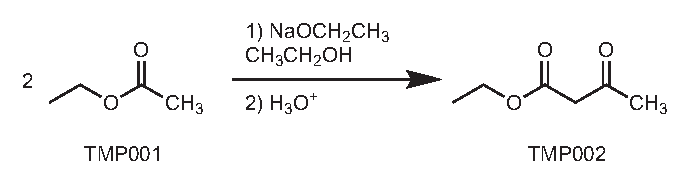
\includegraphics{figures/scheme1.eps}
	\caption{Ester \CNref{ester} gets converted into \CNref{claisenProduct} in a Claisen condensation.}
	\label{sc:scheme1}
\end{scheme}

Also, sublabels can be used. 
See \ref{fig:figure1} for an example.
\ref{fig:figure1} shows benzene (\CNlabelsub{aromatic}{a}) and toluene (\CNlabelsub{aromatic}{b}). % When using sublabels, use the command \CNlabelsub{}{}; the second curly bracket is filled with the sublabel a, b, ...

\begin{figure}
	\centering
	\schemerefsub[TMP003]{aromatic}{a} % When using sublabels in figures or schemes, use the command \schemerefsub[TMPXXX]{}{}; the second curly bracket is filled with the sublabel a, b, ...
	\schemerefsub[TMP004]{aromatic}{b}
	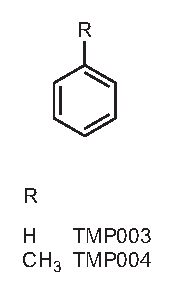
\includegraphics{figures/figure1.eps}
	\caption{If the R group is a hydrogen, this compound is benzene (\CNrefsub{aromatic}{a}). If it is a methyl group, the compound is toluene (\CNrefsub{aromatic}{b}).}
	\label{fig:figure1}
\end{figure}

When adding the TMPXXX labels to a figure and exporting the figure as .eps file (text needs to be exported as text and not as vector graphic), the automatic compound numbering can also be applied there (\ref{fig:figure2}). Hypothetical spectra of compounds \CNlabel{ester}, \CNlabel{claisenProduct}, \CNlabelsub{aromatic}{a} and \CNlabelsub{aromatic}{b} are shown in \ref{fig:figure2}.

\begin{figure}
	\centering
	\schemeref[TMP001]{ester}
	\schemeref[TMP002]{claisenProduct}
	\schemerefsub[TMP003]{aromatic}{a}
	\schemerefsub[TMP004]{aromatic}{b}
	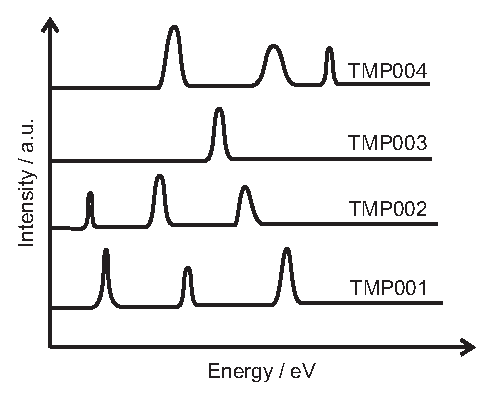
\includegraphics{figures/figure2.eps}
	\caption{Spectra of compounds \CNref{ester}, \CNref{claisenProduct}, \CNrefsub{aromatic}{a} and \CNrefsub{aromatic}{b}.}
	\label{fig:figure2}
\end{figure}

\end{document}